\chapter{Software Testing and Evaluation}
\label{chap5}

To assess the quality of implementation, ensuring each component of this project works properly has top priority, and then the different input settings should be explored. Therefore, this chapter covers the unit test and performance evaluation to prove that the project satisfied the requirements of the initial objectives.

\section{Unit Test}

The unit test needs to verify several components: basic model rendering, GUI update and SDF.

\subsection{External Libraries}

Most of the components are implemented based on several third-party libraries. For example, the model class use the vector definition from the GLM library to store the vertices. Therefore, all libraries should ensure that they are imported correctly so that further programming and testing tasks.

\hspace*{\fill}

GLFW and GLAD testing can be verified through an executable rendering window. Once the libraries are appropriately set, the rendering pipeline is built automatically so that the GPU will render the correct image. GLM and tinyobjloader are required to be adequately included in the source code, and both can be verified through read-in a simple mesh like a cube and converting the object data to the format of GLM; if the code can be compiled and running correctly, both libraries are successfully imported. Similarly, the Dear ImGui library's import status can be verified by rendering a simple GUI component to the application window.

\hspace*{\fill}

Figures \ref{impl:gui} and \ref{impl:modelrender} have proven that the rendering pipeline, GUI library, and obj loader library have been imported properly.

\subsection{Model Rendering}

The application is supposed to process arbitrary obj files. Therefore, both simple and complex meshes are tested for this component, including the simple cube, sphere meshes and common 3D models like Spot, Stanford Bunny and Stanford Lucy. All test models can be read-in and rendered correctly through polygonal and coloured mode.

\hspace*{\fill}

The result of model rendering testing for different meshes is shown in figure \ref{ut:model}.

\begin{figure}[htbp]
    \centering
    
    \subfigure[Cube]{
    \begin{minipage}[t]{0.325\linewidth}
        \centering
        
\includegraphics[width=1.5in]{Images/Chap5/cube_p.png}
        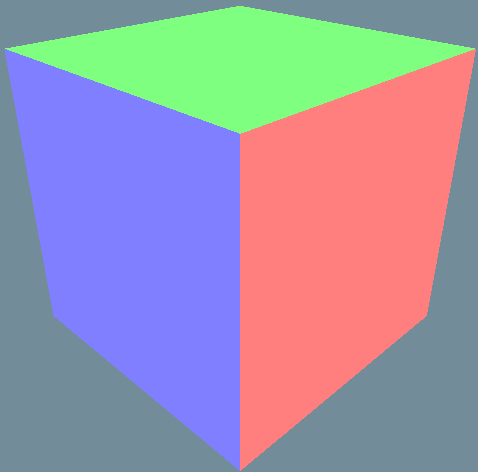
\includegraphics[width=1.5in]{Images/Chap5/cube_c.png}
    \end{minipage}%
    }%
    \subfigure[Sphere]{
    \begin{minipage}[t]{0.325\linewidth}
        \centering
        
\includegraphics[width=1.5in]{Images/Chap5/sphere_p.png}
        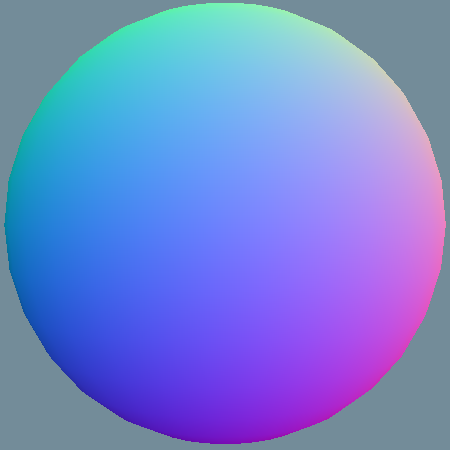
\includegraphics[width=1.5in]{Images/Chap5/sphere_c.png}
    \end{minipage}%
    }%
    \subfigure[Stanford Bunny]{
    \begin{minipage}[t]{0.325\linewidth}
        \centering
        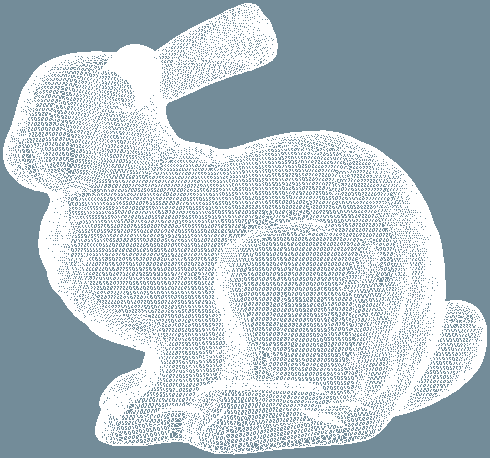
\includegraphics[width=1.5in]{Images/Chap5/bunny_p.png}
        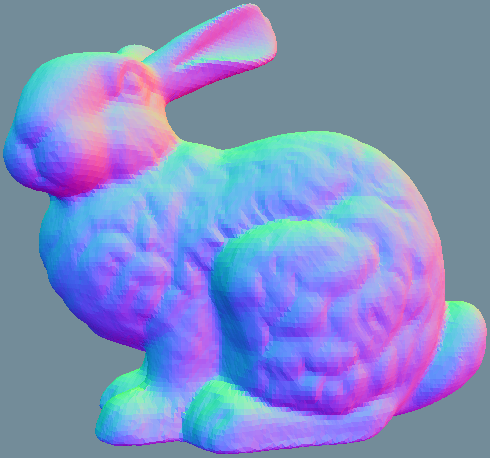
\includegraphics[width=1.5in]{Images/Chap5/bunny_c.png}
        %\caption{fig2}
    \end{minipage}
    }%
    
    \quad
    
    \subfigure[Spot]{
    \begin{minipage}[t]{0.5\linewidth}
        \centering
        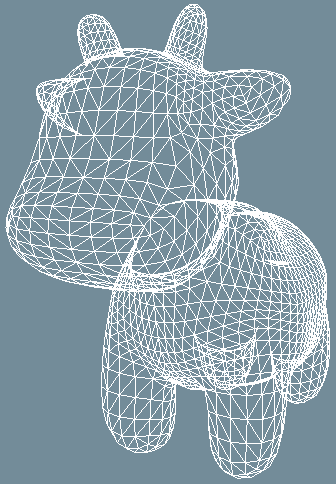
\includegraphics[width=1.5in]{Images/Chap5/spot_p.png}
        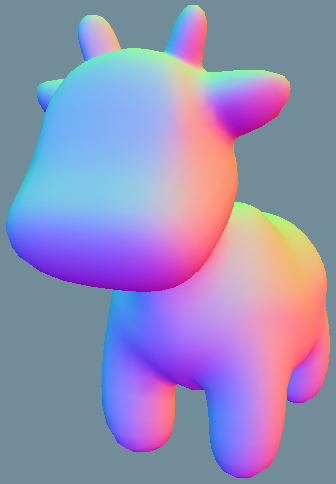
\includegraphics[width=1.5in]{Images/Chap5/spot_c.png}
        %\caption{fig2}
    \end{minipage}
    }%
    \subfigure[Stanford Lucy]{
    \begin{minipage}[t]{0.5\linewidth}
        \centering
        
\includegraphics[width=1.5in]{Images/Chap5/lucy_p.png}
        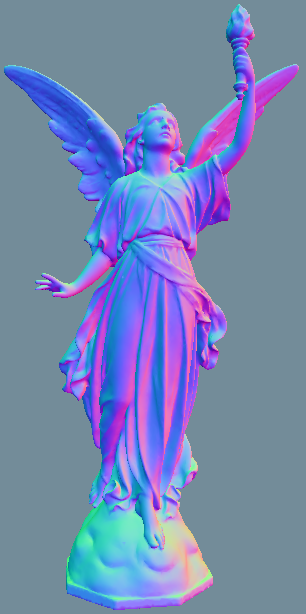
\includegraphics[width=1.5in]{Images/Chap5/lucy_c.png}
        %\caption{fig2}
    \end{minipage}
    }%
    \centering
    \caption{Rendering test for several models}
    \label{ut:model}
\end{figure}

\subsection{GUI update}

Since the computation is time-consuming, the application needs to monitor the progress of computation; the percentage of the whole model computation is shown in the debug area of the GUI panel. The GUI debug status should keep updating during the process of computing the signed distance field and provide a hint when it is finished. 

\clearpage

The GUI panel updates the computation status properly and provides the rendering hint when the computation is finished, as shown in figure \ref{ut:guiupdate}.

\begin{figure}[htbp]
    \centering
    \subfigure[Update]{
    \begin{minipage}[t]{0.495\linewidth}
        \centering
        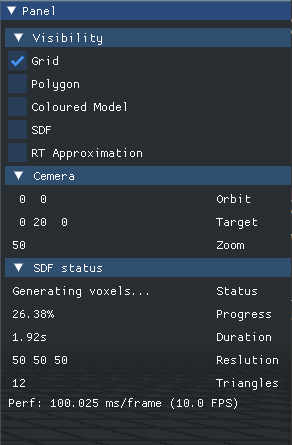
\includegraphics[width=3in]{Images/Chap5/GUIupdate.png}
    \end{minipage}%
    }%
    \subfigure[Sphere]{
    \begin{minipage}[t]{0.495\linewidth}
        \centering
        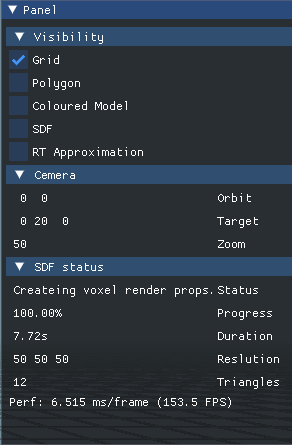
\includegraphics[width=3in]{Images/Chap5/GUIfinish.png}
    \end{minipage}%
    }%
    \caption{The Debug status update properly}
    \label{ut:guiupdate}
\end{figure}

\subsection{SDF}
\label{eva:sdf}

If the SDF has been calculated, the application reads in the generated SDF file to visualize the signed distance field. As shown in \ref{impl:sdfvisual}, the field of Stanford Bunny can be visualized properly. The result of other models can be seen in figure \ref{ut:sdfsphere}, \ref{ut:sdfspot} and \ref{ut:sdflucy}. The effect of different parameter settings on the quality of the SDF is discussed in \ref{eva:quality}.

\begin{figure}[htbp]
    \centering
    \subfigure[Colour Volume]{
    \begin{minipage}[t]{0.245\linewidth}
        \centering
        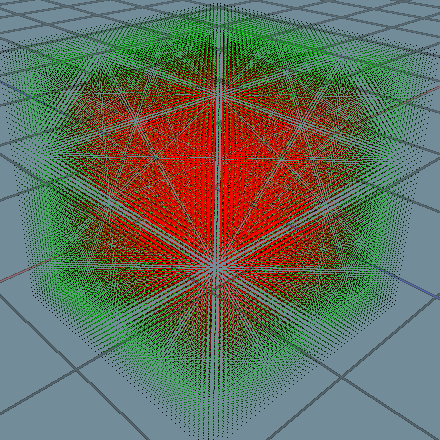
\includegraphics[width=1.3in]{Images/Chap5/cubeiso.png}
    \end{minipage}%
    }%
    \subfigure[Ray Tracing]{
    \begin{minipage}[t]{0.245\linewidth}
        \centering
        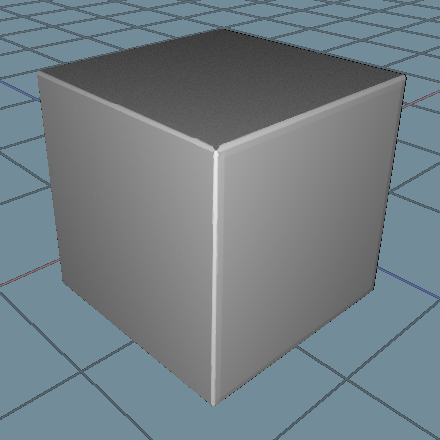
\includegraphics[width=1.3in]{Images/Chap5/cubert.png}
    \end{minipage}%
    }%
    \subfigure[Colour Volume]{
    \begin{minipage}[t]{0.245\linewidth}
        \centering
        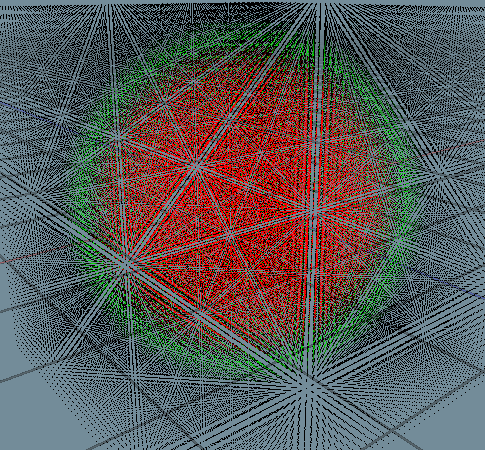
\includegraphics[width=1.4in]{Images/Chap5/sphereiso.png}
    \end{minipage}%
    }%
    \subfigure[Ray Tracing]{
    \begin{minipage}[t]{0.245\linewidth}
        \centering
        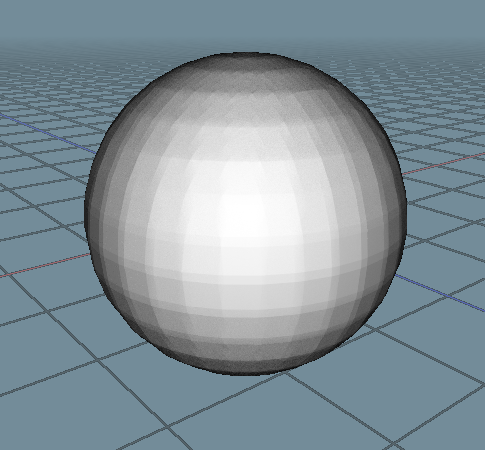
\includegraphics[width=1.4in]{Images/Chap5/spherert.png}
    \end{minipage}%
    }%
    \caption{The SDF visualization of Cube(a,b) and Sphere(c,d)}
    \label{ut:sdfsphere}
\end{figure}


\begin{figure}[htbp]
    \centering
    \subfigure[Colour Volume]{
    \begin{minipage}[t]{0.495\linewidth}
        \centering
        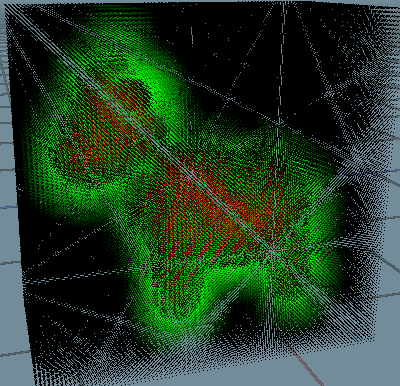
\includegraphics[width=3in]{Images/Chap5/spotiso.png}
    \end{minipage}%
    }%
    \subfigure[Ray Tracing Approximation]{
    \begin{minipage}[t]{0.495\linewidth}
        \centering
        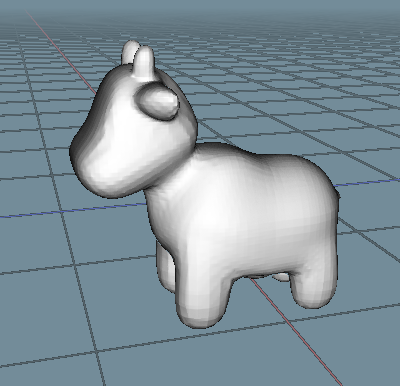
\includegraphics[width=3in]{Images/Chap5/spotrt.png}
    \end{minipage}%
    }%
    \caption{The SDF visualization of Spot}
    \label{ut:sdfspot}
\end{figure}

\begin{figure}[htbp]
    \centering
    \subfigure[Colour Volume]{
    \begin{minipage}[t]{0.495\linewidth}
        \centering
        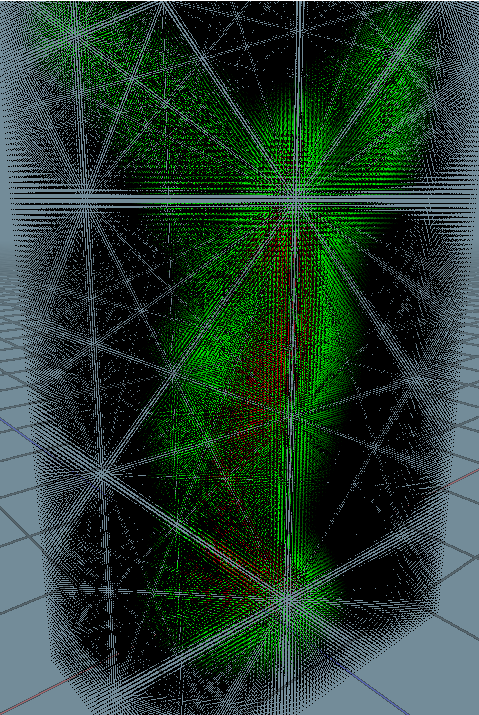
\includegraphics[width=3in]{Images/Chap5/lucyiso.png}
    \end{minipage}%
    }%
    \subfigure[Ray Tracing Approximation]{
    \begin{minipage}[t]{0.495\linewidth}
        \centering
        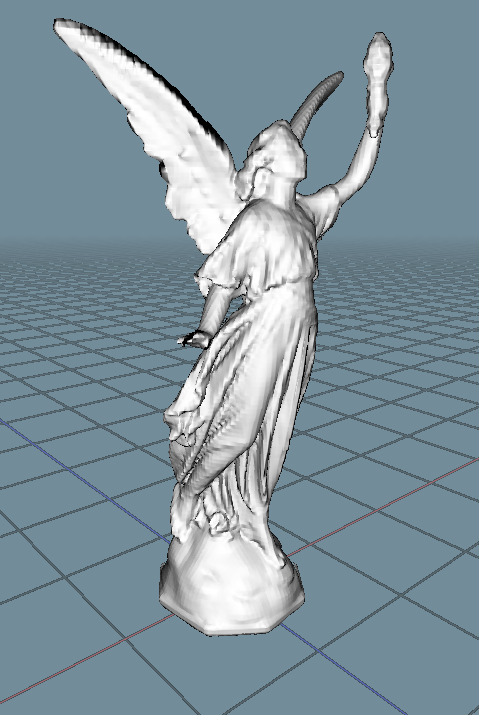
\includegraphics[width=3in]{Images/Chap5/lucyrt.png}
    \end{minipage}%
    }%
    \caption{The SDF visualization of Stanford Lucy}
    \label{ut:sdflucy}
\end{figure}

\clearpage

\section{Evaluation}

Three parameters influence the quality and generation performance of the SDF. The first one is the number of sample rays in each voxels. Another one is the resolution, which influence the number of sample voxels. The last one is triangle number of the mesh. The effect of these three parameters will be explored.

\subsection{SDF quality}
\label{eva:quality}

\subsubsection{Sample Ray Number}

The number of sample rays for each voxel affect the accuracy of distance function computation, if the ray is sparse, then the error of distance value for each sample voxel can be serious. Figure \ref{eva:rayquality} provides the SDF approximation results in different ray number settings, the resolution is set as 50*63*64.

\begin{figure}[htbp]
    \centering
    \subfigure[16 Rays]{
    \begin{minipage}[t]{0.445\linewidth}
        \centering
        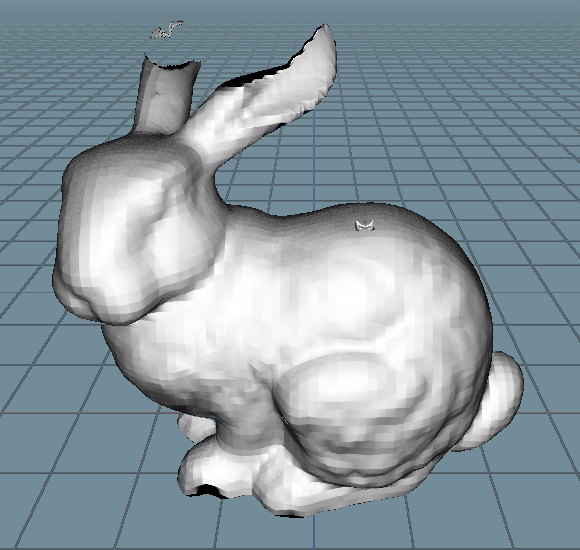
\includegraphics[width=2in]{Images/Chap5/bunny50ray16.png}
    \end{minipage}%
    }%
    \subfigure[32 Rays]{
    \begin{minipage}[t]{0.445\linewidth}
        \centering
        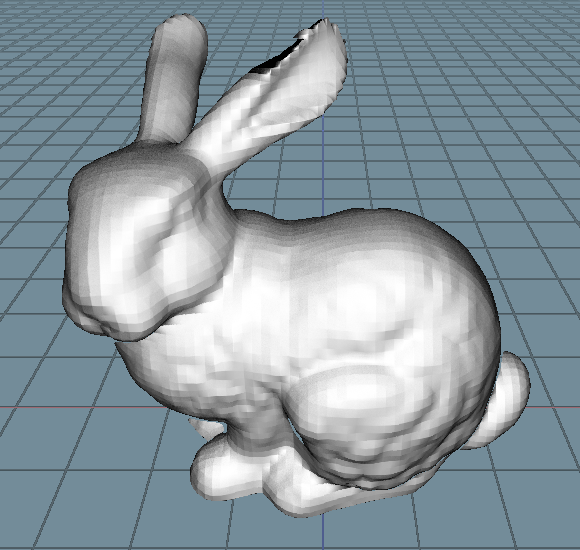
\includegraphics[width=2in]{Images/Chap5/bunny50ray32.png}
    \end{minipage}%
    }%
    \quad
    \subfigure[64 Rays]{
    \begin{minipage}[t]{0.445\linewidth}
        \centering
        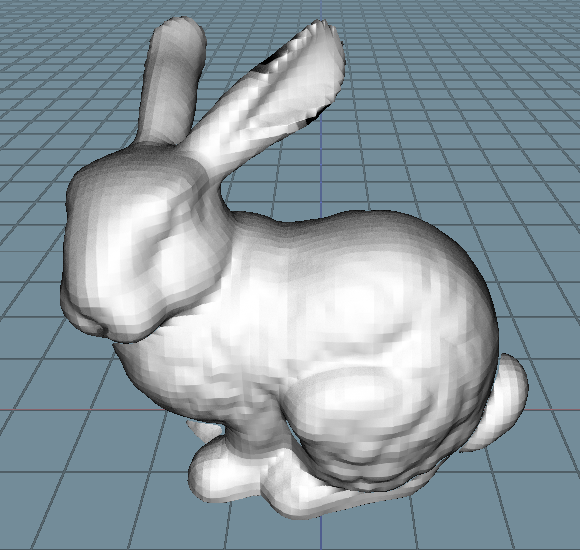
\includegraphics[width=2in]{Images/Chap5/bunny50ray64.png}
    \end{minipage}%
    }%
    \subfigure[128 Rays]{
    \begin{minipage}[t]{0.445\linewidth}
        \centering
        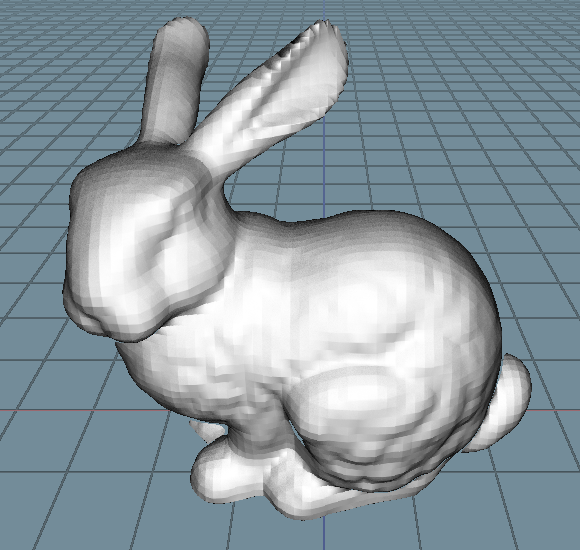
\includegraphics[width=2in]{Images/Chap5/bunny50ray128.png}
    \end{minipage}%
    }%
    \caption{The SDF approximation results for different ray number}
    \label{eva:rayquality}
\end{figure}

As can be seen in figure \ref{eva:rayquality}, when the ray number is low (a,b), there are obvious gaps in the parts of bunny'ears. As the number of rays increases, the error gradually disappears and the shape of Stanford Bunny has been nicely reproduced. Therefore, with a rational setting of ray number, the qualify of SDF generation meets the requirement.

\clearpage

\subsubsection{Resolution}

A high quality signed distance field can be generated with more sample voxels. However, using more sampled voxels can significantly increase the amount of computation and increase the generation time, especially for CPU implemented projects. In this section, the Stanford Bunny is used to explore the influence the effect of resolution on the quality of the generated SDFs since it is one of the most common 3D test model and can easily compare with other's work. The ray tracing visualisation mode is used to show the result.

\begin{figure}[htbp]
    \centering
    \subfigure[10*12*12]{
    \begin{minipage}[t]{0.325\linewidth}
        \centering
        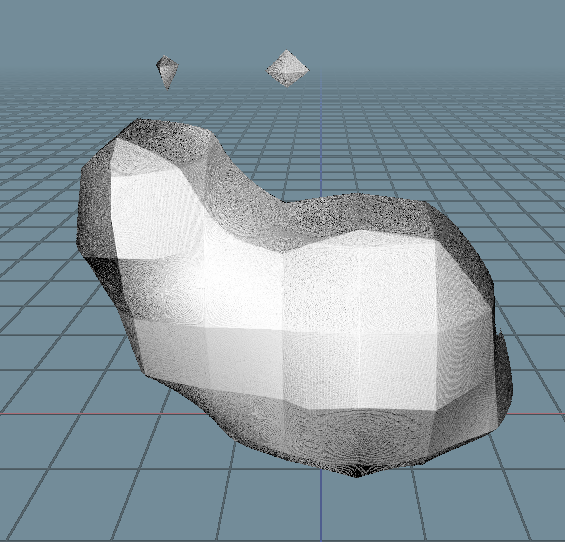
\includegraphics[width=1.9in]{Images/Chap5/bunny10.png}
    \end{minipage}%
    }%
    \subfigure[25*31*32]{
    \begin{minipage}[t]{0.325\linewidth}
        \centering
        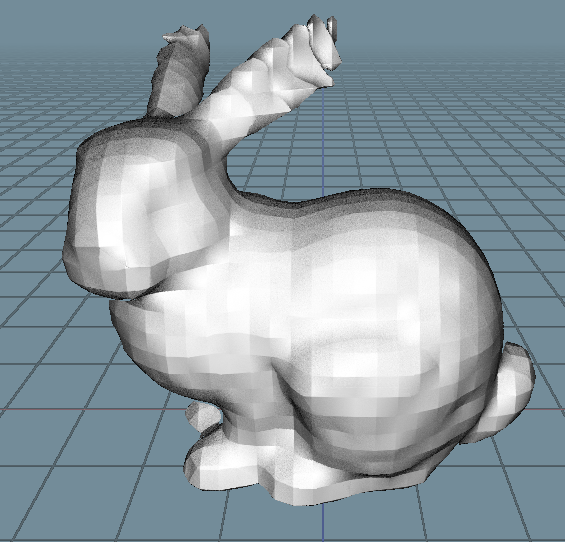
\includegraphics[width=1.9in]{Images/Chap5/bunny25.png}
    \end{minipage}%
    }%
    \subfigure[50*63*64]{
    \begin{minipage}[t]{0.325\linewidth}
        \centering
        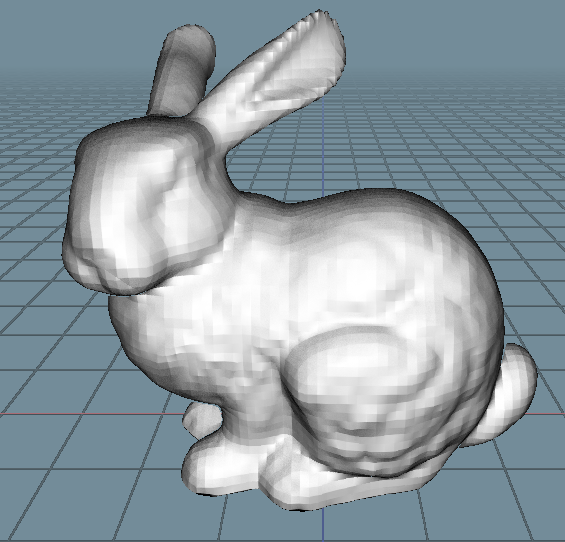
\includegraphics[width=1.9in]{Images/Chap5/bunny50.png}
    \end{minipage}%
    }%
    \quad
    \subfigure[120*153*154]{
    \begin{minipage}[t]{0.475\linewidth}
        \centering
        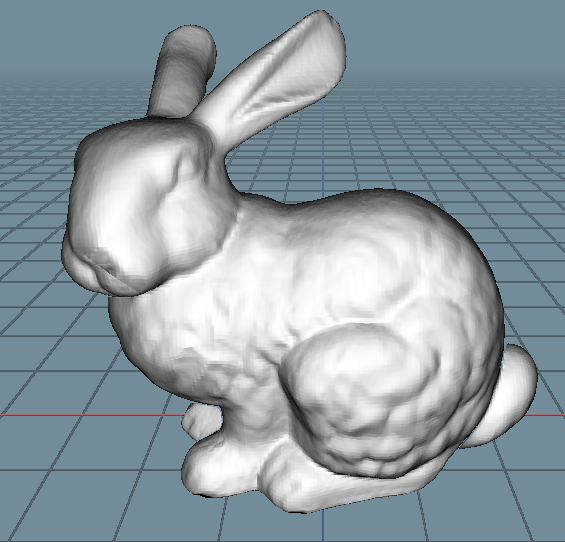
\includegraphics[width=2.45in]{Images/Chap5/bunny120.png}
    \end{minipage}%
    }%
    \subfigure[DeepSDF \cite{park2019deepsdf}]{
    \begin{minipage}[t]{0.475\linewidth}
        \centering
        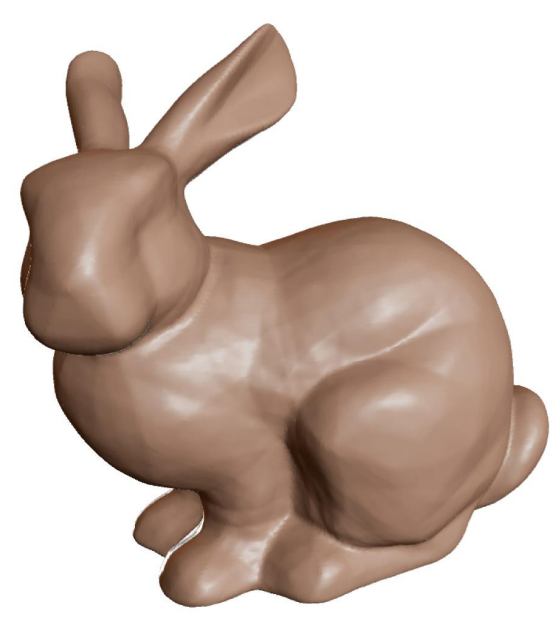
\includegraphics[width=2.15in]{Images/Chap5/bunnyDeep.png}
    \end{minipage}%
    }%
    \caption{The SDF approximation results for different resolutions and comparison with DeepSDF \cite{park2019deepsdf}}
    \label{eva:resquality}
\end{figure}

As shown in figure \ref{eva:resquality}, the shape can be roughly reproduced with a resolution of 25*31*32. The recover result of DeepSDF \cite{park2019deepsdf} is more smooth but lose a lot of details like the fur balls. Conversely, when setting the voxel number on the shortest axis as 120, the most details of the Stanford Bunny mesh can be recovered. Therefore, the quality of SDF is satisfying in this resolution.

\clearpage

\subsection{Performance}

This section will explore the influence of resolution, sample ray number and mesh triangle number on the generation performance. The evaluation has experimented on the computer of the School of Computing.

\hspace*{\fill}

The configuration of the testing computer is as follows:

\hspace*{\fill}

\begin{tabular}{ll}
    CPU & Intel 11th Gen Core i7-11700 2.5GHz\\
    RAM & 32GB DDR4 3200MHz\\
    GPU &  NVIDIA GeForce RTX 3080\\
    OS & Windows 10 Enterprise x64 20H2
\end{tabular}

\subsubsection{Sample Ray Number}

The cube with 12 triangles is used to test the influence of the sample ray number since the influence of the triangle number can be avoided in this setting. The number of sample voxels is set as 6.4k to show the change in generation time. The results can be seen in figure \ref{eva:rayper}.

\begin{figure}[htbp]
    \centering
    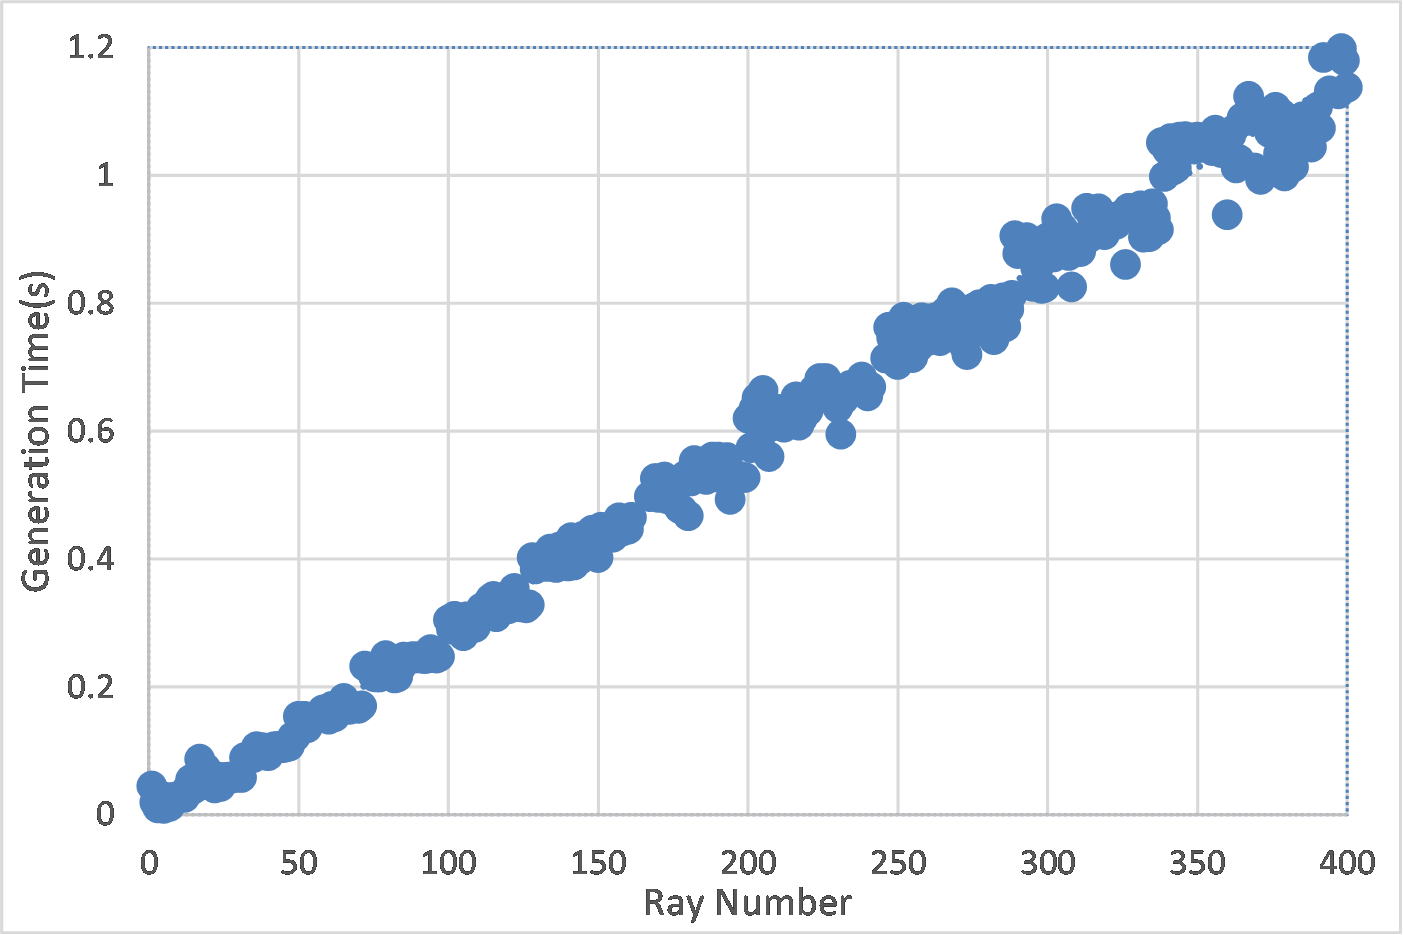
\includegraphics[width=14cm]{Images/Chap5/Ray.png}
    \caption{Generation time results with various ray number}
    \label{eva:rayper}
\end{figure}

As shown in figure \ref{eva:rayper}, the generation time rises linearly as the ray number increases. Therefore, the generation time is only related to the number of rays for each sample voxel when other parameters are unchanged.

\subsubsection{Resolution}

The resolution influence is tested through common 3D models: SPhere, Spot, Stanford Bunny and Stanford Lucy, while the ray number is set as 64 per voxel. The results can be seen in figure \ref{eva:resper}.

\begin{figure}[htbp]
    \centering
    \subfigure[Sphere]{
    \begin{minipage}[t]{0.485\linewidth}
        \centering
        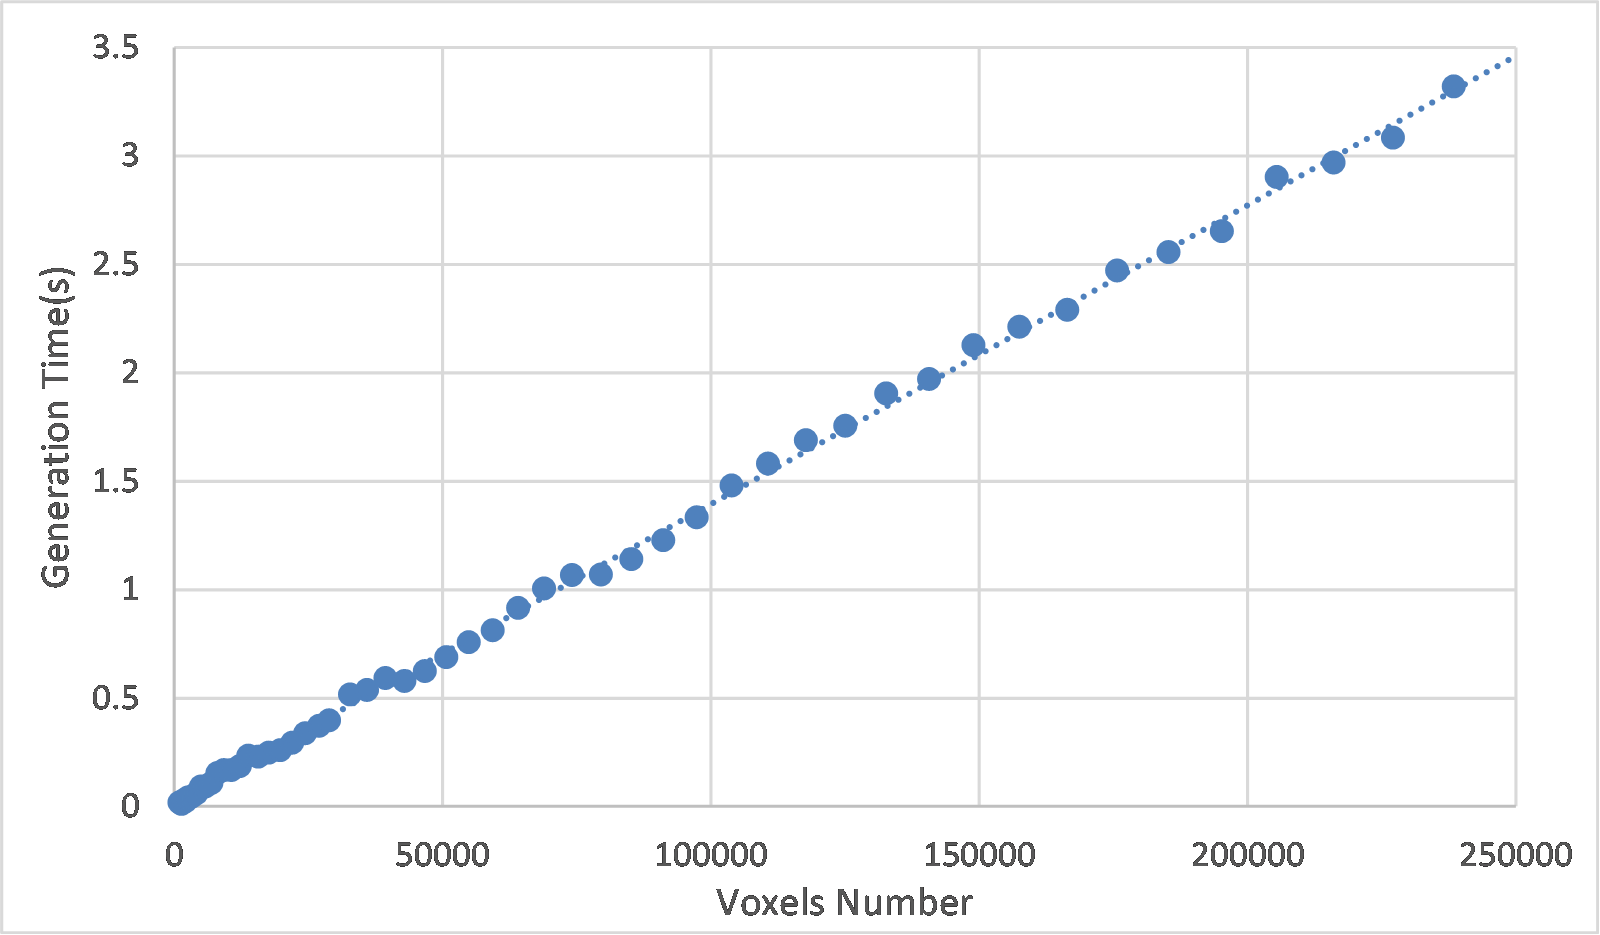
\includegraphics[width=3in]{Images/Chap5/ResSphere.png}
    \end{minipage}%
    }%
    \subfigure[Spot]{
    \begin{minipage}[t]{0.485\linewidth}
        \centering
        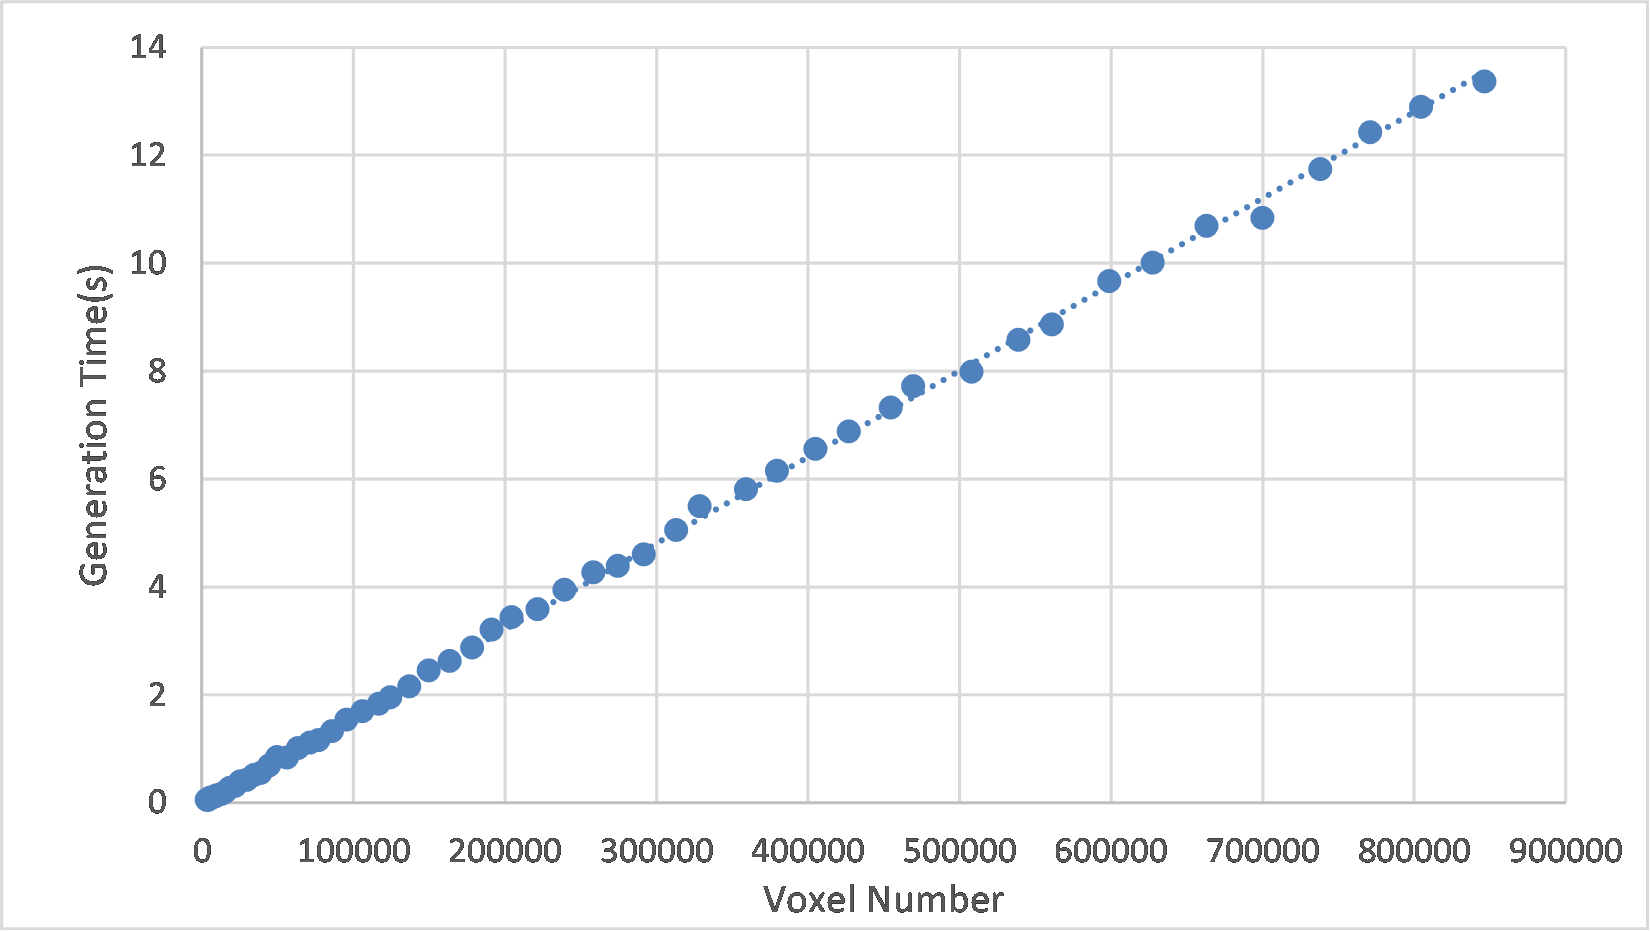
\includegraphics[width=3in]{Images/Chap5/ResSpot.png}
    \end{minipage}%
    }%
    \quad
    \subfigure[Stanford Bunny]{
    \begin{minipage}[t]{0.485\linewidth}
        \centering
        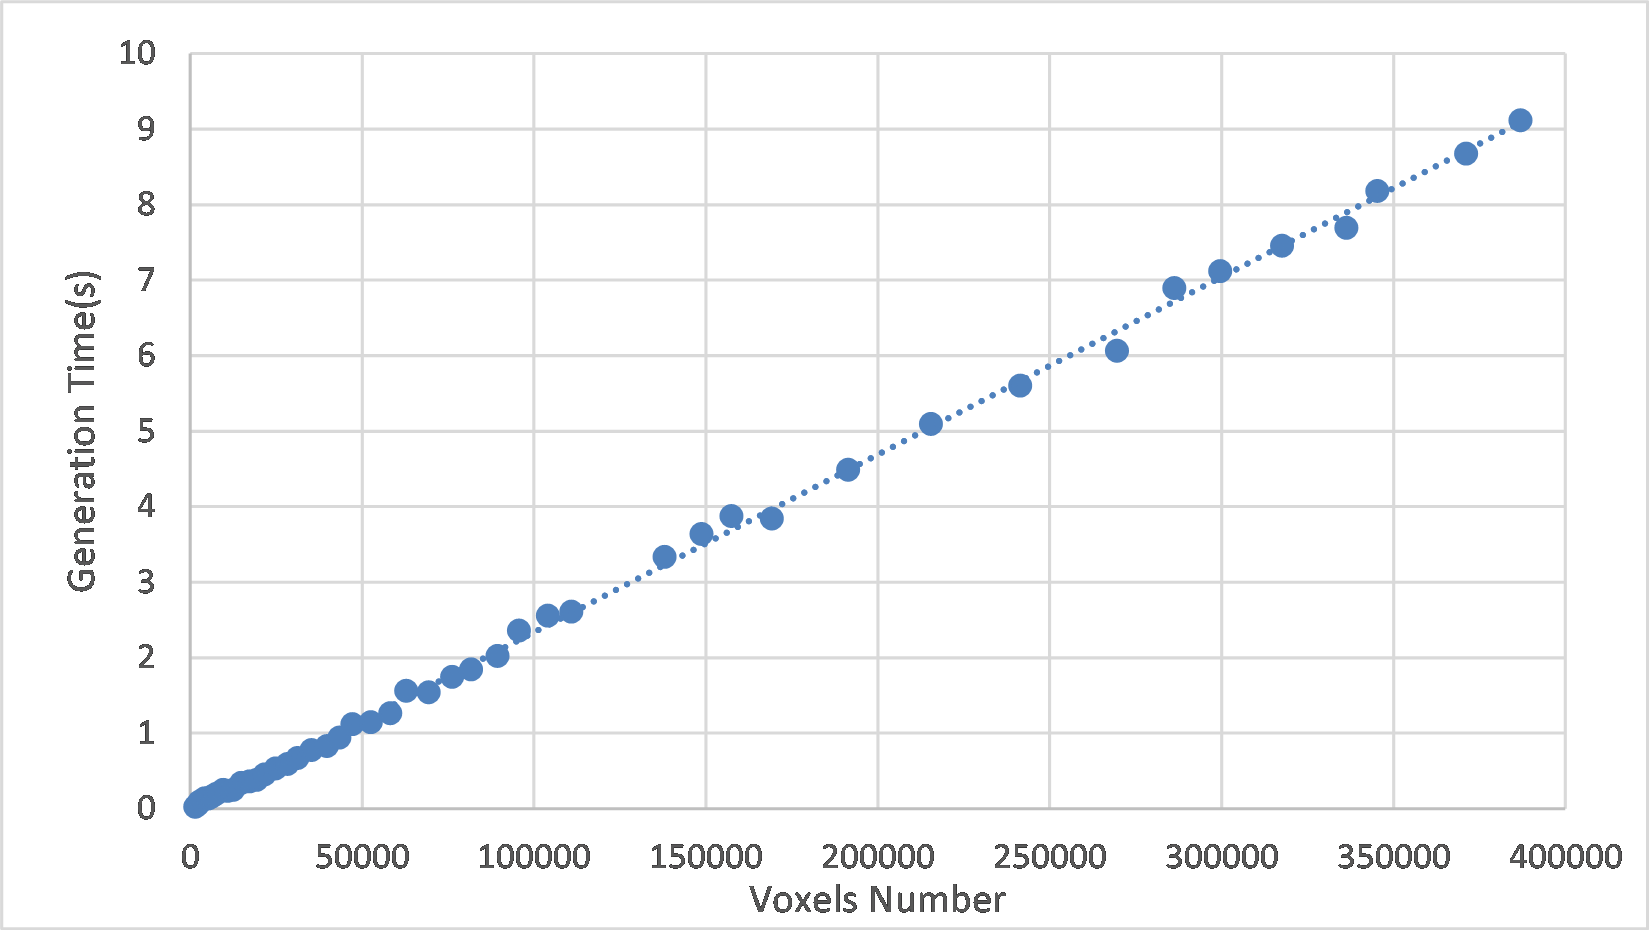
\includegraphics[width=3in]{Images/Chap5/ResBunny.png}
    \end{minipage}%
    }%
    \subfigure[Stanford Lucy]{
    \begin{minipage}[t]{0.485\linewidth}
        \centering
        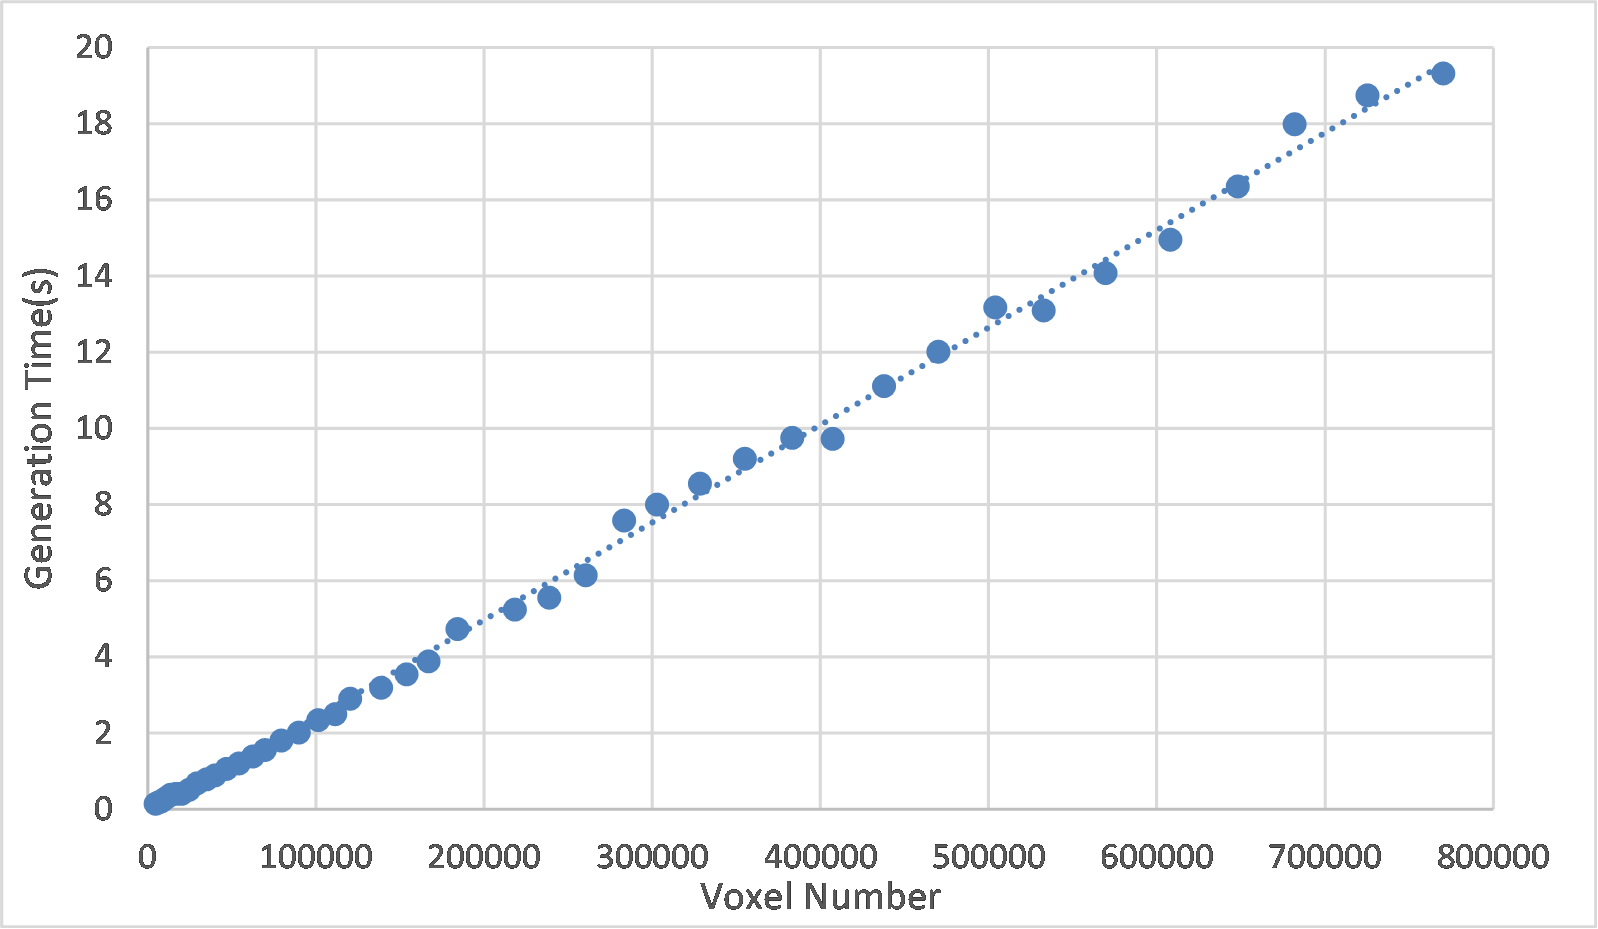
\includegraphics[width=3in]{Images/Chap5/ResLucy.png}
    \end{minipage}%
    }%
    \label{eva:resper}
\end{figure}

As shown in figure \ref{eva:resper}, as the voxel number increase, the SDF generation time experience a linear growth. At this point, the generation time is only positively correlated with the number of voxels. Besides, as seen from the figure, generating the SDF with around 800 thousand sample voxels can be finished within 20 seconds.

\subsubsection{Mesh Triangle Number}

The sphere meshes with different numbers of triangles are used to test the influence of mesh triangle numbers, which can avoid the influence of model shape. The sphere with 1k, 5.5k, 7.5k, 9k and 13k triangles are used, while the ray number per voxel is still set as 64. The results can be seen in figure \ref{eva:triper}.

\clearpage

\begin{figure}[htbp]
    \centering
    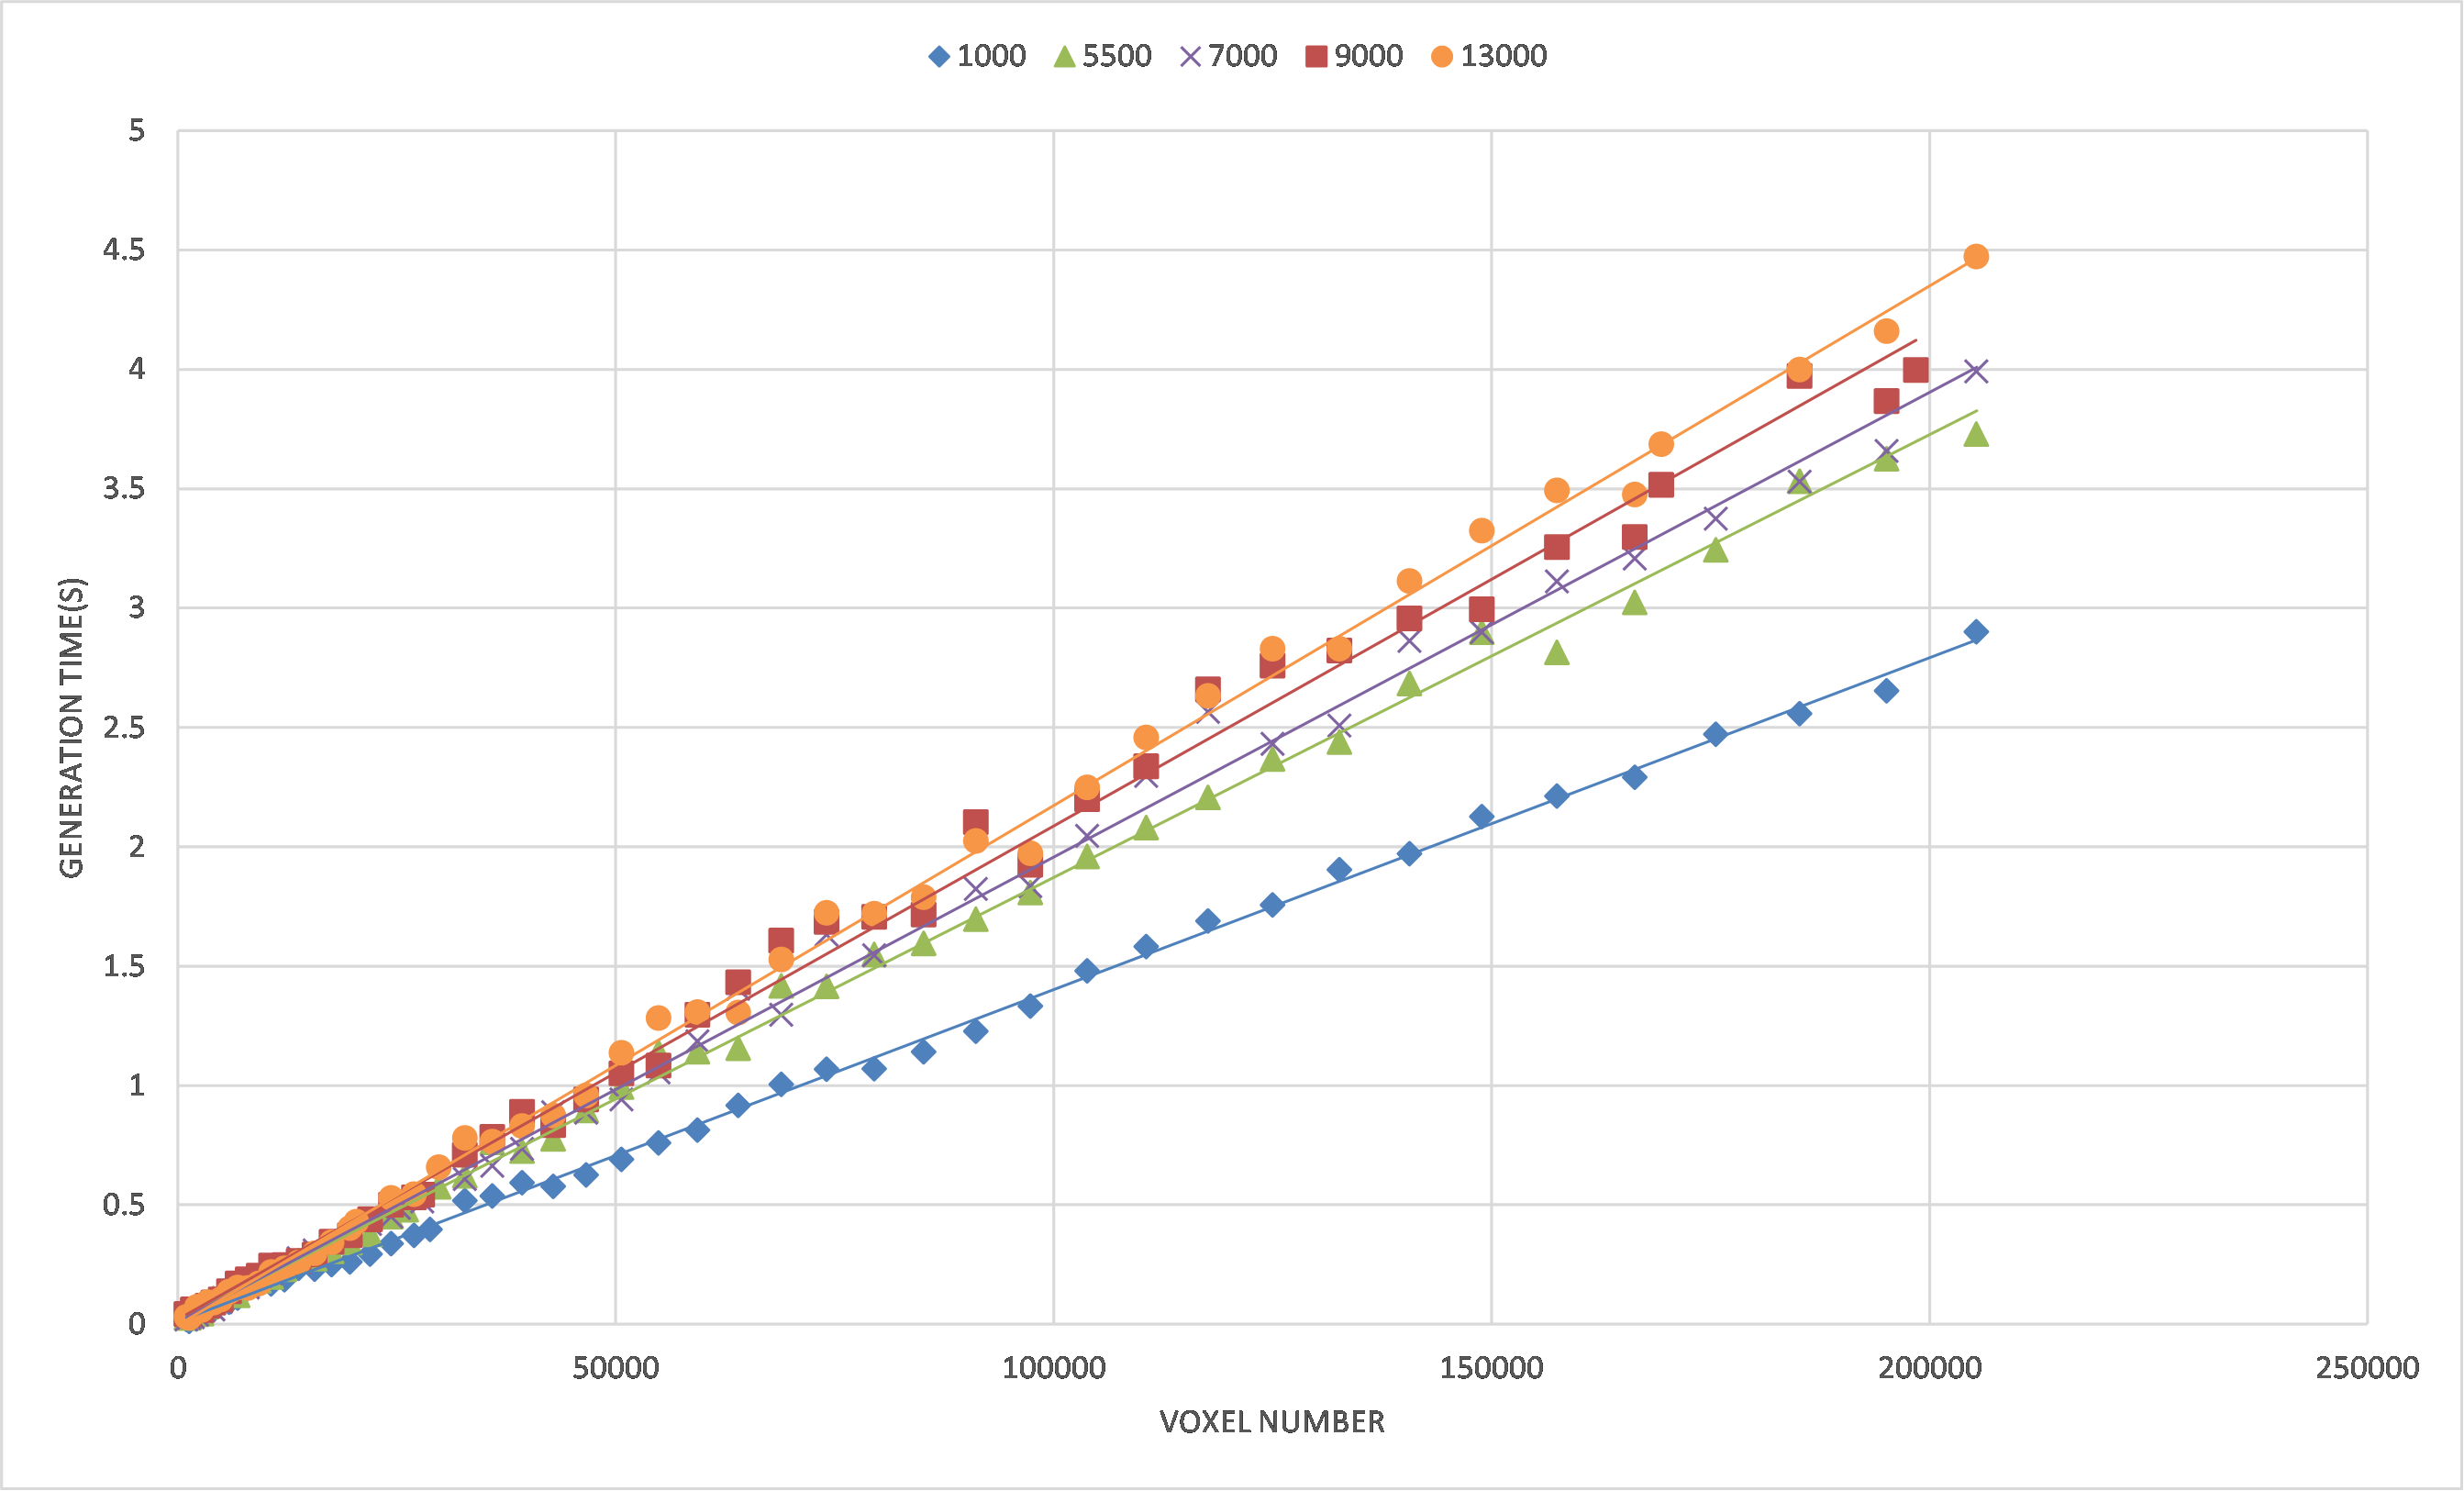
\includegraphics[width=14cm]{Images/Chap5/Triangle.png}
    \caption{Generation time results with various triangle number}
    \label{eva:triper}
\end{figure}

As shown in figure \ref{eva:triper}, the different triangle number affects the slope of the generation time with respect to the number of voxels. For the models with shape, generating an SDF with the same sample voxels cost more time if the mesh triangle number is larger.